% Simulation architecture documentation for the Kassiopeia Guide
\chapter{The \textsc{Kassiopeia} Architecture}\label{ch:architecture}

\section{Global Picture}
\label{arch:globalpicture}

The core of \textsc{Kassiopeia} is made up of pieces of code that fall into three principal categories:  Managers, Modules, and Data Containers.  This architecture is used by the main application (Kassiopeia, for tracking simulations), and other applications within \textsc{Kassiopeia}.  Most of this discussion will focus on the simulation but will be applicable to other applications as well.

The Data Containers are basic objects that simply represent the state of the simulation in computer memory as it is executing, and it is the responsibility of the Modules to initialize and update the contents of these Data Containers as simulation time progresses.  The Managers in turn organize and control which Modules are active at which time.

Managers come in two varieties: Toolboxes and `Execution' Managers.  Toolboxes simply collect and organize available Modules, and Execution Managers connect the Modules in the Toolboxes together and use them to progress the simulation.   

The Data Containers are organized into four physically intuitive levels of detail:  Runs, Events, Tracks, and Steps.  Since it is the job of the Modules and Managers to figure out how to update these Data Containers as time progresses, this organizational principle naturally extends to the rest of \textsc{Kassiopeia}, too.  It is therefore worthwhile to describe in detail how interesting simulation information falls into these four categories.

\section{Simulation Organization}
\label{arch:simorganization}

\subsection{Runs}
\label{arch:runs}

The Run organization level is the highest level, and represents everything that happens during one execution of \textsc{Kassiopeia}.  A Run is not much more than a collection of Events, and global information that only pertains to Runs is limited to the number of events that occur in a run and how much physical time elapsed during the period of the Run.  It is important to note that no physical parameters of the simulation may change during a Run.  This includes but is not limited to high-voltage settings, magnet currents, and the like.  Therefore, the present \textsc{Kassiopeia} definition of Run is in line with the Katrin experimental definition of a Subrun.  Support for real experimental Runs and the consequently necessary name change will be added in a future version.

\subsection{Events}
\label{arch:events}

The Event organization level matches what one would intuitively think: a physical process occurs to generate one or more primary particles, whose states are represented by Tracks, and all of the things that happen as a consequence of these Tracks and their secondary Tracks are grouped together into an Event.  In \textsc{Kassiopeia} there is one type of Module devoted to the creation of the inital state of these primary Tracks, called a Generator.  The name of our package of Generators is KPAGE (KATRIN PArticle GEnerator), and technical details about how these Modules work can be found in the KPAGE section of this document.

\subsection{Tracks}
\label{arch:tracks}

The Track organization level, as alluded to before, represents information about the physical particles that \textsc{Kassiopeia} aims to simulate.  To be precise, in \textsc{Kassiopeia} a Particle is an instantaneous \emph{physical} state of a Track, defined by a position vector, a momentum vector, rest mass, charge, spin, lifetime, and and particle type ID number.  These ID numbers match the PDG standard where defined for particular species.  Tracks in \textsc{Kassiopeia} contain two Particle states each: one for the initial state, and one for the current state which gets updated as the simulation runs.  Tracks also contain additional, non-physical simulation information, including an ID number that is unique and causally sequential within an event, a stamp indicating the physical process that created the Track, and the ID number of a parent Track.  In the case that a particle is primary and directly created by a Generator Module (thus having no parent Track), this ID has the value -1.  Finally, Tracks also have available their path length, their elapsed time, the number of steps used in their calculation, and a stamp indicating the reason \textsc{Kassiopeia} stopped the Track.  In \textsc{Kassiopeia}, the modules associated with the Track level are geometrical objects, called Regions, described in section \ref{arch:geometry}.  These are special Modules that represent user instructions for what physical processes \textsc{Kassiopeia} should simulate.

\subsection{Steps}
\label{arch:steps}

The Step organization level is the finest level of detail considered in \textsc{Kassiopeia}.  A Step is an incremental, discrete change to a Track.  In most applications it has two conceptual parts, the first being the numerical solution to an equation of motion, and the second being the simulation of discrete physical processes that may have occurred during flight along the step.  Steps keep track of their initial physical state, again represented as a Particle, and their final physical state, which, if the Step is acceptable, becomes the most current physical state of the Track to which the Step belongs.  As with the case for Events and their Generators above, \textsc{Kassiopeia} has several types of Modules whose responsibilities fall within the scope of calculating Steps.  The first of these is the Process type of Module, which is responsible for actually calculating the final Particle states within a Step.  Working closely with these Processes is the Step Size type of Module, which cooperate to determine the largest possible time increment over which a set of Processes may accurately act.  The last type of Module working at Step scope is the Exit Condition, which can indicate that a Step is the final one \textsc{Kassiopeia} will calculate for a given Track.  The suite of Processes, Step Sizes and Exit Conditions currently used in Kassopeia are documented in the KTrack section, with the exception of KESS which is a specifically designed process used for tracking in silicon.

\section{Geometry}
\label{arch:geometry}

Geometrical information is of course necessary in any particle tracking simulation.  In \textsc{Kassiopeia}, geometrical information is utilized in two distinct ways.  First, in the more local of the two ways, geometry is used as configuration information for modules.  For instance, field calculation Modules need to know where electrodes and magnets are, or a Generator Module might need to know the dimensions of a container filled with Radon.  In the more global usage, however, \textsc{Kassiopeia} associates configurations of Step level Modules with geometrical objects, essentially mapping out a geometry based plan of how to compute tracks and steps.  As mentioned above, such a binding between a geometrical object and a computation strategy is a special Track-level Module called a Region.

The basic Geometry objects themselves are oriented in a global \textsc{Kassiopeia} coordinate system, and are able to do all purely geometrical calculations required for simulation.  This includes determining whether a point is inside of the object or not, and a computation of the shortest distance to the object from a point.  The shapes available in \textsc{Kassiopeia} are currently limited to truncated cones and cylinders, as cylinders are a special limiting case of truncated cones.  This will be expanded in the next version, as will the calculations available in the Geometry objects in general.

\subsection{Regions}
\label{arch:regions}

A set of Regions in \textsc{Kassiopeia} is always a properly nested set of volumes, meaning that any Region may have sub-Regions which are completely contained within the parent Region without overlapping its boundaries.  Similarly, sub-Regions that are contained inside a parent Region may not overlap either.  This restriction on the geometries defining Regions allows the Regions to be organized in a tree-like way, with a single, special Region at the base of the tree.  This special Region is called the Root Region, and it physically contains all other Regions used and has no parent itself.  The tree structure of the Regions also is the way Regions are represented in the code of \textsc{Kassiopeia}:  each Region can be queried for its parent Region, and also for its set of child Regions.  A picture of a properly nested set of cylindrical Regions and the in-memory representation of this structure appears in figure \ref{archfig:geometry}.

\begin{figure}[!htb]
\centering
\includegraphics[width=0.7\textwidth]{images/ArchitectureFigures/ArchGeometry.pdf}
\caption{The geometrical and in-memory structure of Regions in \textsc{Kassiopeia}}
\label{archfig:geometry}
\end{figure}

The association between Regions and Step-level Module configurations is realized through a programming idea called the Command pattern.  In this pattern, a Command to switch configuration is itself saved, along with the Module being added or the name of the module being removed.  Such a saved Command is in a ready-to-execute state, and may be finally executed at any time, by any part of the code without that code needing to know the details of what the Command does.  This is done for speed reasons, since it saves having to retrieve a stepping Module from the Step Strategy Toolbox every time a configuration change is desired.  This is lookup is rather done one time during \textsc{Kassiopeia}'s execution during the initialization stage.  For each region, these Commands are separated into entry and exit commands, and each type is saved in an ordered list that may be accessed during computation.

\subsection{Navigation}

As a Track is being computed, \textsc{Kassiopeia} needs to know which Region the Track's current Particle state falls inside in order to load the proper Step computation Modules.  This is accomplished using a piece of code called the Navigator, which acts like an iterator for the tree structure of the regions.  As an iterator, it `sits' on the current Region occupied by the Track's Particle, and can travel up and down the branches of the tree structure as the Particle changes Regions as Tracks are updated.  As the Navigator traverses the tree, it builds up an ordered list of Commands to execute when it has completed its journey.

The basic algorithm for Navigation is recursive, and works as follows:

\begin{itemize}
\item The Navigator is given a Track's current Particle's position.
\item The Navigator determines whether this position is inside its current Region.
\item If it is still inside, the Navigator checks to see if the position is also inside one of the current Region's sub-Regions
    \begin{itemize}
        \item If so, the current Region is set to this sub-Region, the entry commands for the sub-Region are added to the list, and the function recurses.
        \item If not, or if there are no further sub-Regions, and the current Region is correct.
    \end{itemize}
\item If it is not still inside, the current Region is set to the parent Region, the exit commands for the old current Region are added to the list, and the function recurses.
\item If the position is outside of the root Region, an error is generated.
\end{itemize}

When the Navigator has finally oriented itself, it will have built up a list of configuration Commands to execute, gathered from nodes in the Region tree.  These Commands are directly executed by the Navigator as soon as the correct Region is found.

\section{CoreManager}
The entire management structure is overseen by the CoreManager (singleton).  The class KSCoreManager is a base class for application-specific derived classes.  For instance, KSCoreManagerSimulation is the CoreManager for the Kassiopeia application (tracking simulations).  Since this is a singleton class, only one CoreManager can exist at any given time.  Creation of the CoreManager is taken care of through the KSManagerFactoryTable.
 
KSCoreManager takes care of setting up the management hierarchy, and reading in the main configuration files.  It initiates the Setup and Prepare processes for all Managers and Toolboxes.  The specific derived CoreManager being used is responsible for specifying what the management structure will be (by choosing its downstream Managers), and performing the executing the actions taken by the application.  Again using KSCoreManagerSimulation as an example, the downstream Managers include KSRunManager, KSGeometryToolbox, KSFieldToolbox, SSCToolbox, KSGeneratorToolbox, KSStepStrategyToolbox, and KSDAQProcessorToolbox.  The Execute method creates and closes the output file, and runs the simulation.
 
The KSExceptionManager and the hierarchical structure of KSExceptionHandlers are responsible for writing log and error messages. They also cleanly handle situations where the simulation needs to shut down due to any sort of error.
 
The DataManager (singleton) is responsible for writing the output data.
 
The Management base class, KSManagerBase, provides the basic functionality common to all managers. These functions include those necessary to build (Setup()), navigate  (Get[Up/Down]streamManager()) and shutdown (ShutDown()) the tree-like management structure.  Furthermore, three other important functions are common to all managers:
\begin{itemize}
 \item Prepare()
 \item ProcessCommand()
 \item Execute()
\end{itemize}
 
Prepare() reads in the module configuration from the default or user-provided configuration file (if applicable), and generally gets the Manager or Toolbox ready for use in the simulation.
 
ProcessCommand() allows requests for configuration changes between managers to happen dynamically during the simulation (e.g. to change the field calculation method when entering another region of the experimental setup).  ProcessCommand() can deal with different types of inputs, given in form of KSBasicCommands, and is used for initialization and for configuration changes during a simulation.
 
Execute() causes the manager to perform its responsibilities on the data that is given as an argument.  Since each manager deals with different types of data, Execute() takes an arbitrary argument in form of a boost::any, and returns another arbitrary argument (again in the form of a boost::any*).  In contrast to KSManagerBase::ProcessCommand, KSManagerBase::Execute should typically only deal with one type of input, although that is not a strict requirement (for the experts: boost::anys provide intrinsic type information, which is its main advantage over void pointers as a solution for this kind of problem).
 
\section{Toolboxes}

Toolboxes are a type of Manager that stores configured Modules of \textsc{Kassiopeia}.  Since they are in the management chain, they are accessible from the CoreManager.  Each type of Toolbox has a configuration file associated with it, in which a user describes in detail a set of related Modules, each of which has a name.  When this configuration file is read, the Initializer/Builder system of \textsc{Kassiopeia} actually instantiates and configures the Modules described, and then registers them inside the Toolbox the system is set to work with. Other pieces of \textsc{Kassiopeia} can then query the Toolbox to retrieve these prepared modules.  Upon exit of \textsc{Kassiopeia}, Toolboxes are finally responsible for deleting all the modules they hold.

There are five types of Toolboxes associated with \textsc{Kassiopeia}:  Geometry, Field, SSC, Generator, and StepStrategy.  

\begin{itemize}

\item The Geometry Toolbox holds all the Geometry information used in calculations in \textsc{Kassiopeia}, as well as the Region modules that map out \textsc{Kassiopeia}'s computation strategy.  The Regions are stored simply by saving the root Region, with the sub-Regions stored directly in their natural tree structure.

\item The Field toolbox holds all the Modules involved in calculating electric and magnetic fields.  These Modules are typically used by other components in carrying out their responsibilities.  For instance, Modules involved in stepping need field information in order to evaluate the equations of motion, and some generators need to know the fields at initial points in order to calculate the momentum of particles.  

\item The SSC toolbox contains components of the SSC package of \textsc{Kassiopeia}, which is used in detailed simulations of the WGTS at Katrin.  SSC can perform detailed calculations of column density, as well as tritium spectra, and is principally used at the Event level of the architecture, but may also be used at the Step level for specific scattering calculations.  For more details, please see the SSC section.

\item The Generator toolbox naturally contains the Modules of \textsc{Kassiopeia} relevant for initializing Events and the Tracks they primarily contain.  There are a wide range of Generators available in \textsc{Kassiopeia}, with sources ranging from electron guns to radioactive volumes of gas. for more details on these and how they are configured, please see the KPAGE section of this document.  

\item The Step Strategy toolbox contains the three module types involved in calculating steps:  Step Sizes, Exit Conditions, and Processes.  These are exclusively used at the Step level to propagate particles.

\end{itemize}

For example, if there is a cone defined in Geometry Configuration file, a corresponding builder will create a cone object and configure it with the user defined values (e.g. radius). Then this object will be stored in the Geometry Toolbox together with other geometry objects. Technically, an add-function is used to store all these geometry objects in a geometry map and can later be accesed easily with a get-function.

In this way, all objects defined in the configuration files are created and placed in the corresponding toolbox.


\section{Rootclasses}

The Rootclasses are very similar to the Toolboxes. But whereas the Toolboxes contain all objects that have been defined in the configuration files, the Rootclasses only contain objects that are actually needed in the region the particle is currently in. So the content of the Rootclasses will be changed while the program is running, whereas the content of the Toolboxes is fixed in the initialization phase of the program. The regions, and the modules that should be used while the particle is inside these regions, can be defined in the \textsc{Kassiopeia} configuration file.

For example, all exit conditions that have been defined in the configuration files will be stored in the Step Strategy Toolbox. If a particle now enters a region, where the user only wants to use one of these exit conditions and has defined this in the \textsc{Kassiopeia} configuration file, the ExitCondition Rootclass will only content this object. Therefore, the function to check the exit conditions will automatically only check for this one.

But how will the content of the Rootclasses be changed while the program is running? After each step there will be a check if a new region has been entered or the current one has been left. In this case, a list of entry/exit commands, that have been created by the navigator (see chapter \textit{navigation} will be executed to change the content of the Rootclasses.


\section{Run, Event, Track, Step Managers}

Each level of the organizational structure in \textsc{Kassiopeia} has an associated Manager, referred to in the introductory paragraph as `Execution' Managers.  These managers drive simulation computation at their associated level.  Typically, the manager of a higher level will be responsible for creating an instance of the class used and filled in by a Manager of a lower level.  This is necessary because of the encapsulated nature of the architecture:  A manager of one level is responsible for calculating the contents of that object in isolation of other objects of the same type.  Therefore sequential id numbers of, say, Tracks can only be known at the overstanding Event level.

A pattern for the operation of these Managers occurs throughout the hierarchy (with a modification at the Step level done for speed).  First, an overstanding Manager creates an object of the type beneath it in the hierarchy, assigning it any sequential ids as necessary.  It then hands the prepared object to the next Manager type, which completely calculates the object it was given.  This process repeats itself until the original overstanding manager has created and completed all the objects it needs to have finished the object it was orignally given by its overstanding manager.  At the end of an object's calculation, it is told to write itself down, if configured to, by the manager that created it.  Finally, it is deleted.

The optimizing exception noted above for the case of the Step Manager is due to the typically very large number of Steps per Track in \textsc{Kassiopeia}.  At this level, the Track Manager makes a single Step object per Track it is given, then re-uses this Step object throughout the calculation of the current Track.

\section{Initialization}

\section{Output}
\begin{DoxyAttention}{Attention}
The source of this documentation can be found in: /KSCore/Main/KSCoreManager.h. some links will not work in the UserGuide, because there targets only exist in the ReferenceGuide.
\end{DoxyAttention}
The standard format for all output data is the \hyperlink{namespace_r_o_o_t}{ROOT} TTree. The output TTrees are stored in a TFile.

The output falls into three categories: \char`\"{}configuration\char`\"{}, \char`\"{}truth\char`\"{} and \char`\"{}real.\char`\"{}

The \char`\"{}configuration\char`\"{} data contains all the user specifications. That is necessary, because some if the configuration options may be set with the command line. However it is currently not existent, so you better keep track of your simulations....

The truth data includes all of the simulation-\/side information. This includes all information about all particles that were simulated, regardless of whether were actually \char`\"{}detected.\char`\"{}

The real data replicates what would be seen in an actual data file. It uses the same TTree format, and only includes information about detected events. Since the DAQ simulation is currently not functional, there is no real data tree in the \hyperlink{class_kassiopeia}{Kassiopeia} output files.

Two types of truth data are recorded: \char`\"{}physics\char`\"{} events and \char`\"{}DAQ\char`\"{} events. These are recorded in separate trees. Again, however, since the DAQ simulation is currently not functional, only the TTree of physics events is recorded.

The truth-\/side physics data can be written out in one of two different standardized formats, both of which reflect the event/track/step hierarchy. The output format is specified in the GlobalConfiguration file. 
\begin{DoxyItemize}
\item {\bfseries TClonesArray}: the TFile consists of a TTree of KMCEvents, which also include track and step data by using TClonesArrays. This is the standard output format, and it's faster than the ThreeTrees format. 
\item {\bfseries ThreeTrees}: the TFile consists of three trees, one for event, one for track and one for step data. This is primarily useful for simulations with large numbers of steps (e.g. trapped-\/particle studies), and as a more convenient format if you want to use the TTreeViewer in \hyperlink{namespace_r_o_o_t}{ROOT}. Otherwise it is slower than the TClonesArray format. 
\end{DoxyItemize}

The classes used to save the various blocks of data are different than the main KSEVent/KSTrack/KSStep classes. The output classes are called KMCEvent, KMCTrack, and KMCStep. The data are stored in blocks classes are KMCEventData, KMCTrackData, and a few different things for the steps.

The internal structure of the KMCEvent is rather non-\/intuitive, since for performance reasons during the saving, the data blocks inside an event have to have fixed size. A step in \hyperlink{class_kassiopeia}{Kassiopeia} is a rather complicated thing -\/-\/ different data may need to be saved depending on the active stepper and its internal state. Therefore the design of the output file structure has been challenging.


\begin{DoxyImage}
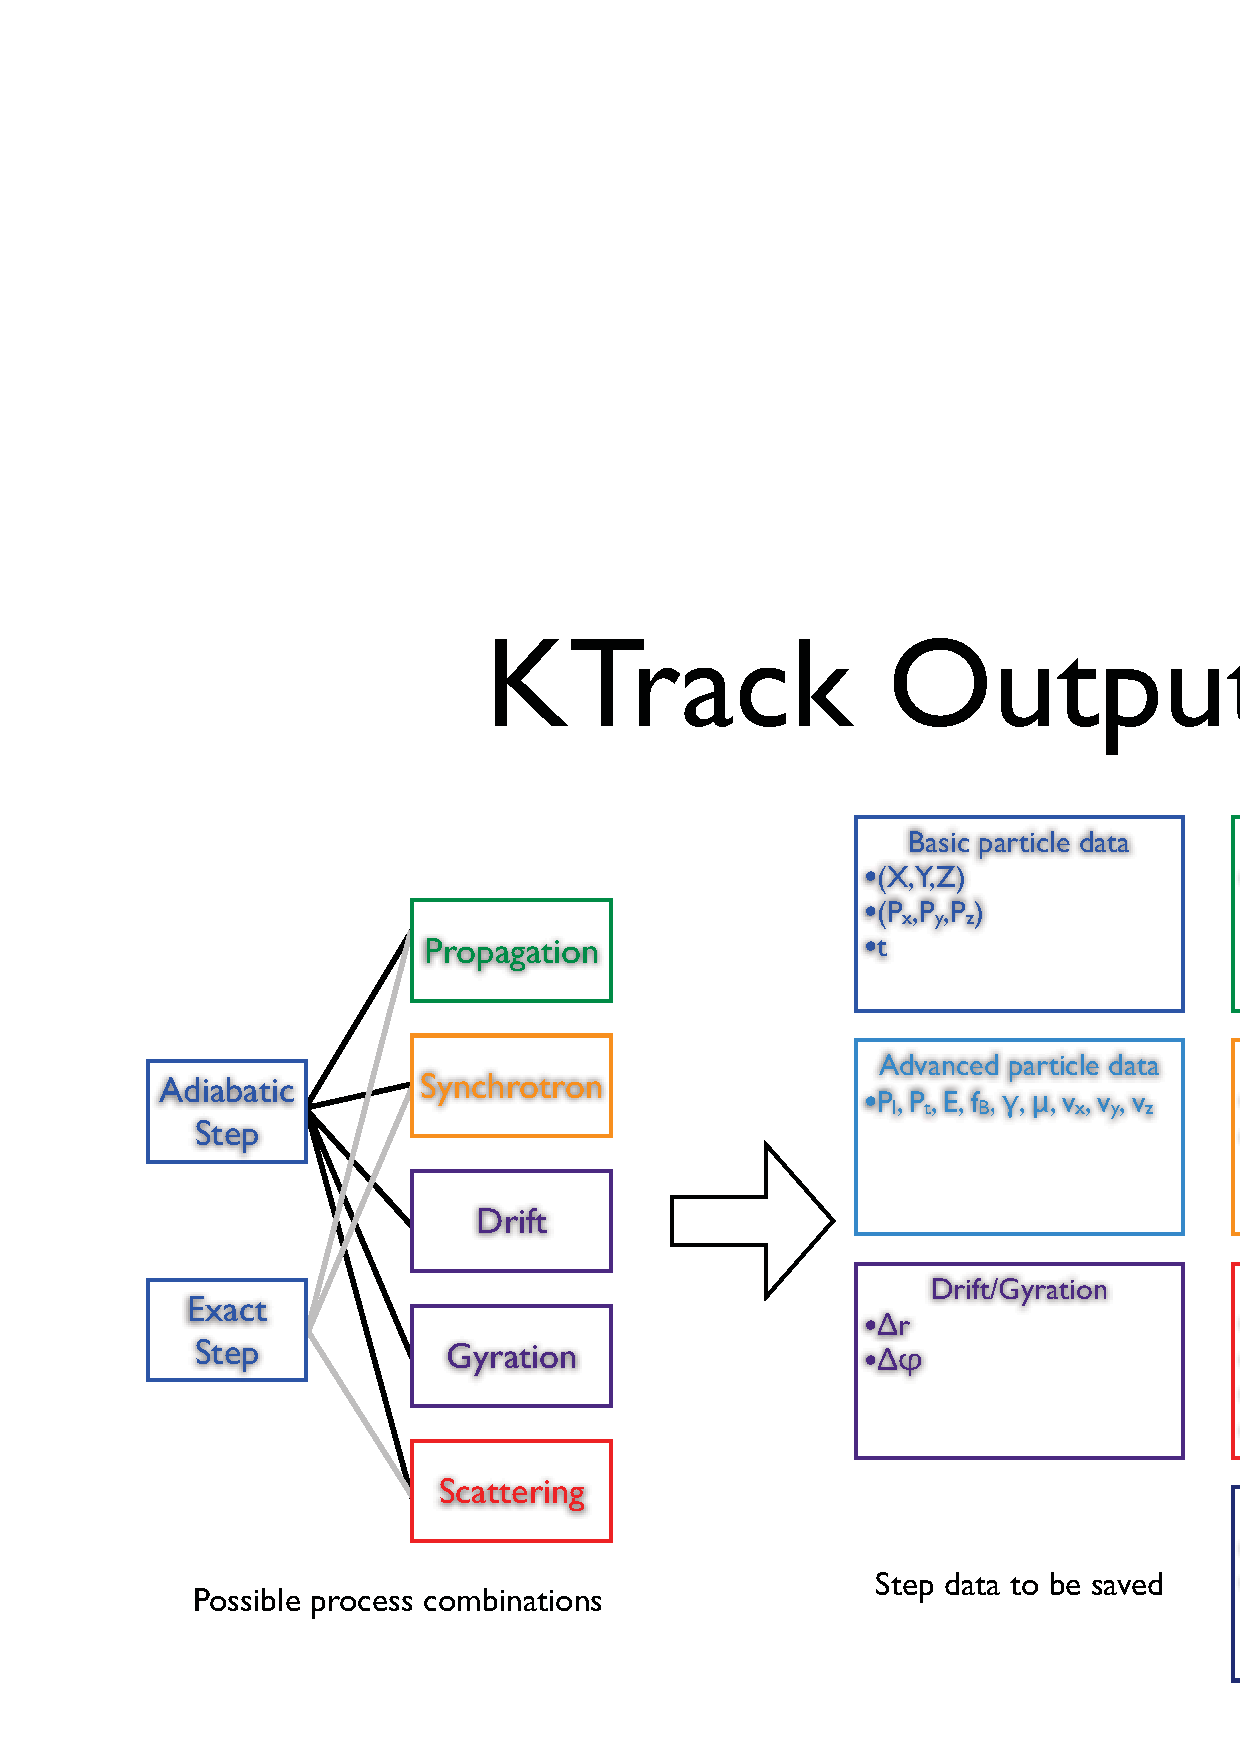
\includegraphics[width=\textwidth]{images/Output_fig1}
\caption{Tracking Step Output}
\end{DoxyImage}
 

The KMCStep class is special in the sense that its size in memory can change from one step to the next. e.g. you may chose to save scattering information only if a scattering interaction actually took place, or a process can be switched of and thus stop providing data altogether. For this reason, the step itself is split up in different fixed size blocks when it is written to disk and the KMCStep again has a non-\/trivial substructure. It consists of several Data blocks, which may or may not be present, and it's Save function knows how to deal with that. Simultaneously, it has a ReadNextStep block for accessing each step recursively. Note that the KMCStep class is strictly speaking not necessary, since it is not written to disk. it is only provided to encapsulate the complex step structure of a step within it.

The event structure as it is written to file is depicted in Fig.2: An event consists of an array of fixed sized blocks for the Track data, and presently eight fixed sized blocks which may of may not be written during each step. In order to retrieve a step from the track, the Trackdata block also contains a two-\/layered key system allowing the retrieval of step information. This key scheme is explained in the following figures:


\begin{DoxyImage}
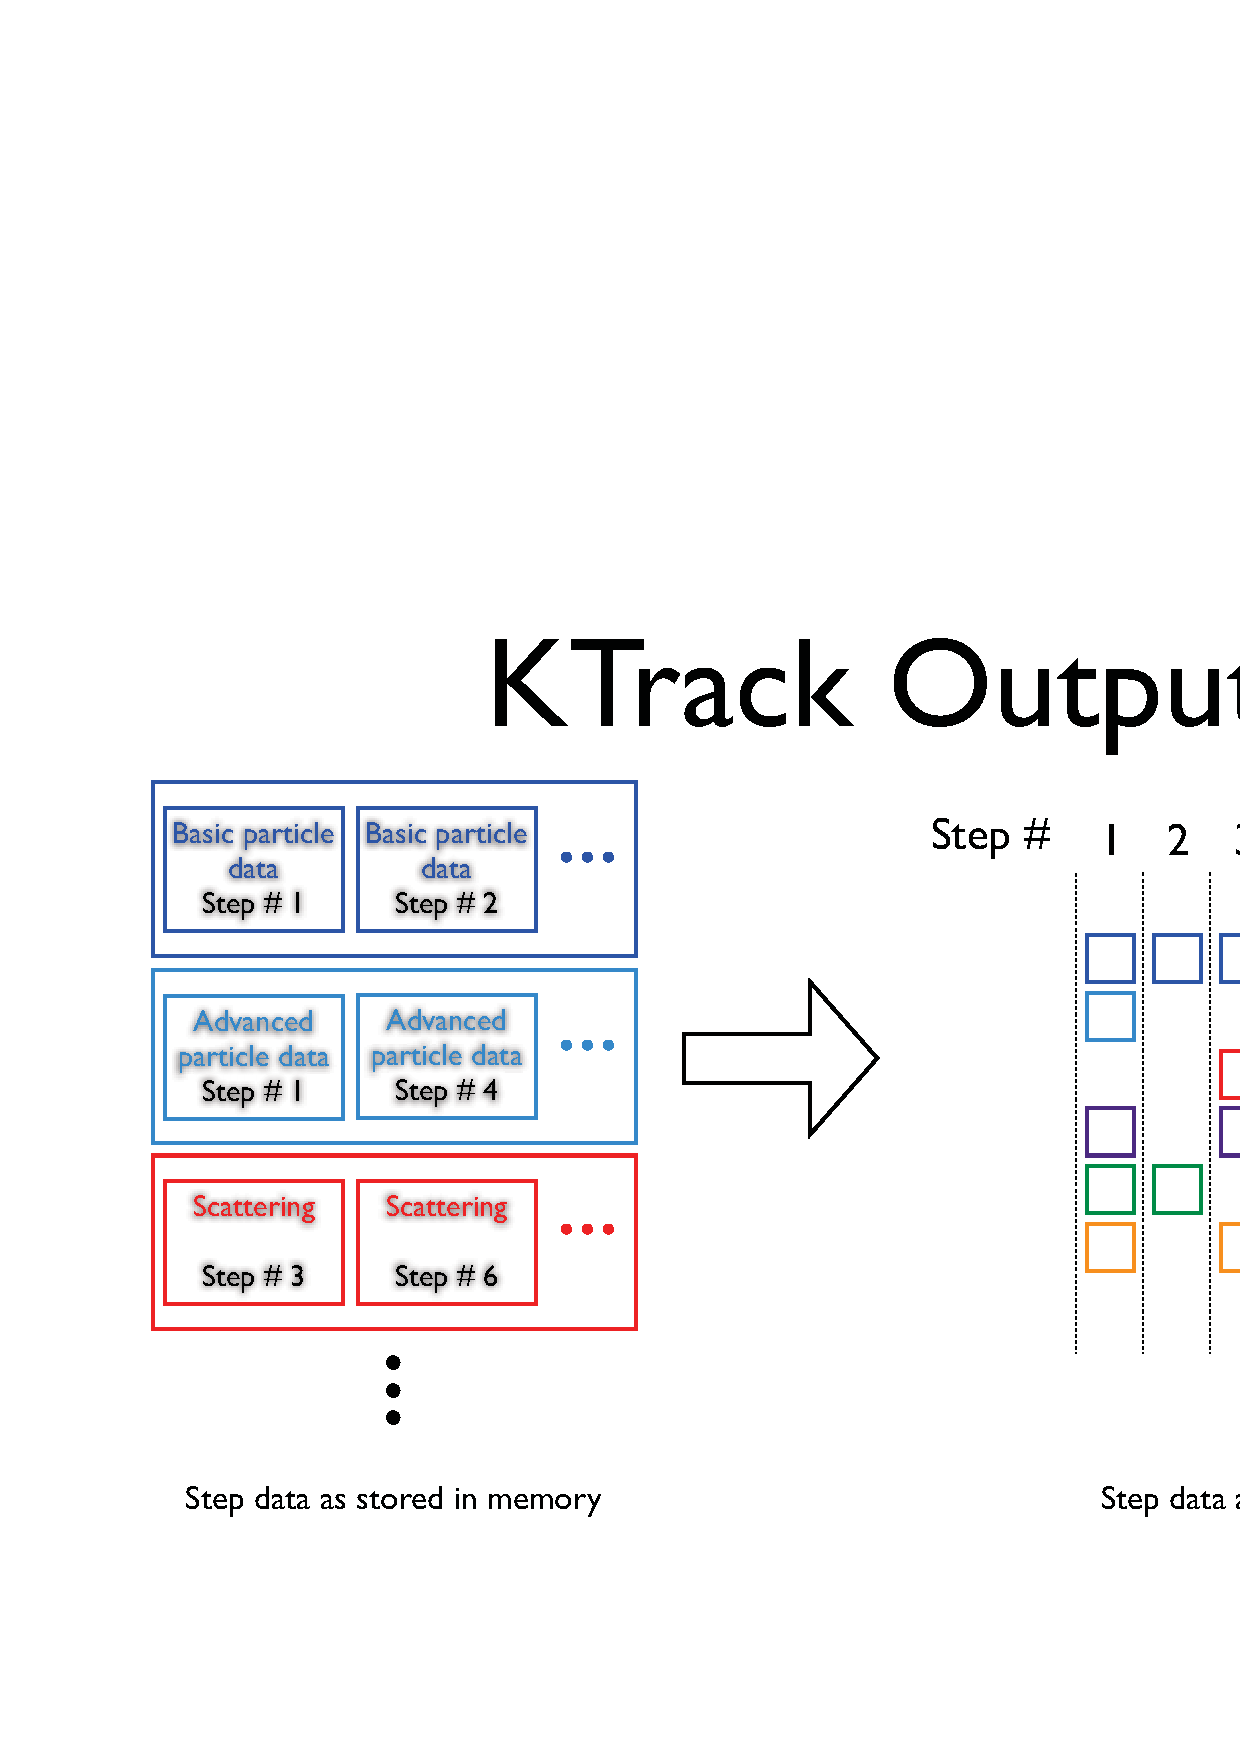
\includegraphics[width=\textwidth]{images/Output_fig2}
\caption{Step Keys scheme}
\end{DoxyImage}
 


\begin{DoxyImage}
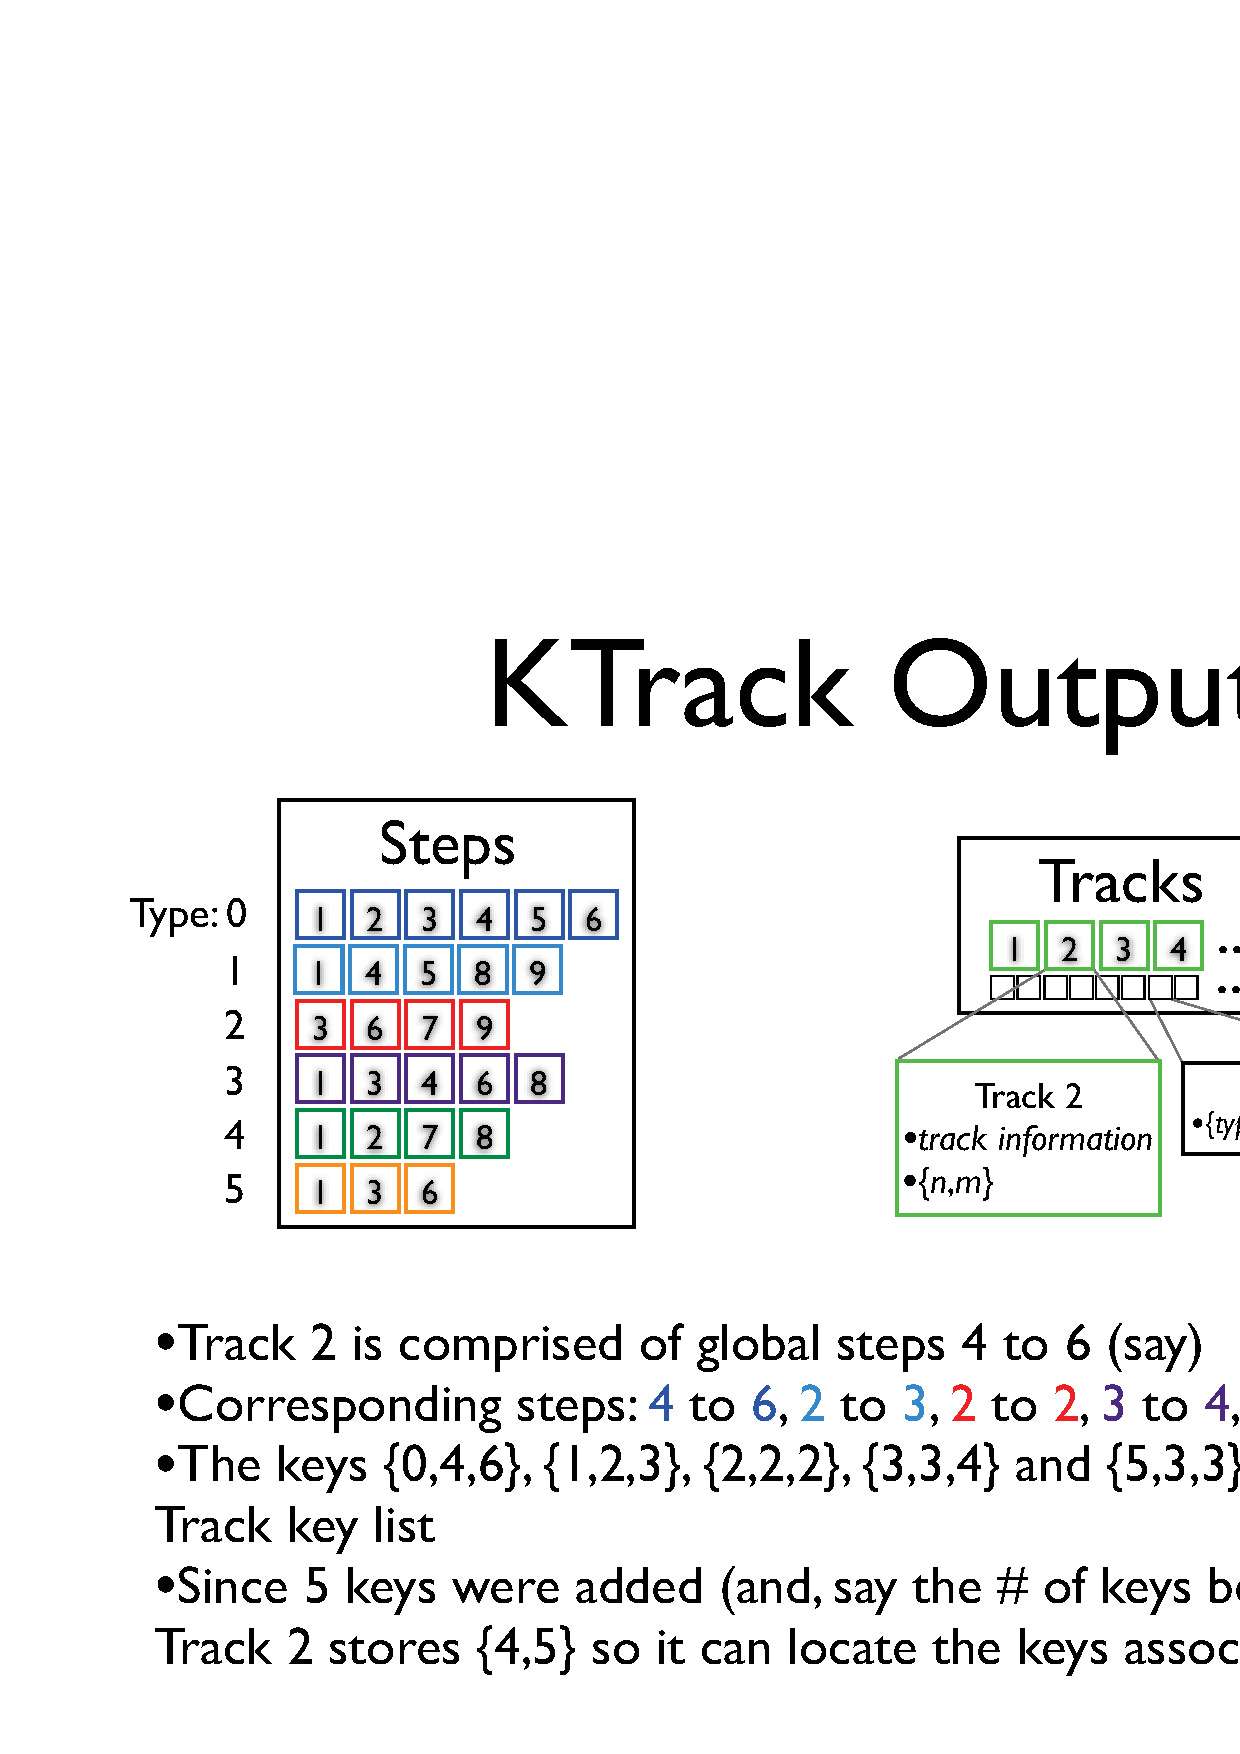
\includegraphics[width=\textwidth]{images/Output_fig3}
\caption{Step Keys example}
\end{DoxyImage}
 

In order to ensure accessibility of the data at all times, the output classes have a version ID provided by the \hyperlink{namespace_r_o_o_t}{ROOT} object IO system. If their design changes, this version number will have to be increased.\hypertarget{_k_s_output_KSAnalysis}{}\subsection{Analysis}\label{_k_s_output_KSAnalysis}


 \hypertarget{_k_s_output_KSTools}{}\subsubsection{existing tools}\label{_k_s_output_KSTools}
As an extremely preliminary general analysis tool, the macro FileReader.C is installed in the binary folder. It can be used as follows: First of all, start root. Then in root do: 
\begin{DoxyCode}
      root [0] .L /path/to/kassiopeia/bin/FileReader.C
      root [1]  FileReader("/path/to/filename", "/path/to/kassiopeia/lib);
\end{DoxyCode}
 The intension of that macro is that the user adjusts it to suite his purposes. That is the main reason why it is provided as a \hyperlink{namespace_r_o_o_t}{ROOT} macro, not a compiled binary. Apart from missing header inclusions, the code in the macro compiles. So if you want to compile your own analysis code, the following piece of code shows how to read the output. It is a one to one copy from the macro FileReader.C. Make sure to read the section about linking to kassiopeia. This code works regardless of the file format, although it is to some extend experimental. Note that the the Filereader macro gets overwritten everytime you do make install, so you better rename it. It's original source code can be found in Application/Macros...


\begin{DoxyCode}
  Kassiopeia::KMCDataManager* myManager = 
      Kassiopeia::KMCDataManager::GetInstance();
  myManager->OpenFile(argv[1],0);
  Kassiopeia::KMCEventIterator* myevent2 = myManager->GetEvent();
  //unitilized pointer to event data, does not contain any useful information at 
      this point

  for (UInt_t ievent = 0; ievent < myManager->GetNEvents(); ievent++){
      myManager->ReadNextEvent(); //now we load the event data of the next event.
      
      Kassiopeia::KMCTrackIterator* mytrack2 = myevent2->GetTrack();
      for (UInt_t itrack = 0; itrack < myevent2->GetNTracks(); itrack++){
          myevent2->ReadNextTrack();
          Kassiopeia::KMCStepIterator* myStep2 = mytrack2->GetStep();
          for (UInt_t istep = 0; istep < mytrack2->GetNSteps(); istep++){
              mytrack2->ReadNextStep();
          }
      }
  }
\end{DoxyCode}
 Additionally, a program called Trackplotter is installed, which plots the geometry and tracks of a simulation.\hypertarget{_k_s_output_KSlinking}{}\subsubsection{Linking}\label{_k_s_output_KSlinking}
In case you want to link your own code against kassiopeia, you can use the 'pkg-\/config'utility to print the compiler and linker flags using 
\begin{DoxyCode}
 pkg-config --cflags kassiopeia
 pkg-config --libs kassiopeia
\end{DoxyCode}
 in the command line or rather your makefile. pkg-\/config is a general tool, its purpose is similar to the root-\/config utlity you probably know. The way this works is that \hyperlink{class_kassiopeia}{Kassiopeia} installs a file called libkassiopeia.pc. This file tells pkg-\/config the necessary information so that it can print the linker options. For this to work, pkg-\/config must find this file! That either requires that you install kassiopeia in a default place like /usr/, or that you add the directory containing kassiopeia.pc (@/@/pkg-\/config) to the environment variable PKG\_\-CONFIG\_\-PATH.\hypertarget{_k_s_output_KSdynamicLoading}{}\subsubsection{Dynamic loading of kassiopeias output classes in ROOT}\label{_k_s_output_KSdynamicLoading}
Another small little feature which might come in handy: \hyperlink{class_kassiopeia}{Kassiopeia} installs a file called libkassiopeia.rootmap. This file tells root in a CINT session (i.e. the root command line), which libraries it needs to load if it encounters kassiopeias classnames. CINT will then try to do that. Of course it only works, if root finds the rootmap file and the library. I haven't found any explicit documentation where \hyperlink{namespace_r_o_o_t}{ROOT} searches for these files, but it seems to look for bith in the current directory, default places like /usr/lib, the root library directory probably LD\_\-LIBRARYPATH.

You can check whether \hyperlink{namespace_r_o_o_t}{ROOT} knows the kassiopeia DataStructure classes by opening a simulation output file in root, e.g. by passing it as argument to root, when starting it. in that case, you could directly use 
\begin{DoxyCode}
    Kassiopeia::KMCDataManager* myManager = 
      Kassiopeia::KMCDataManager::GetInstance();
\end{DoxyCode}
 and the following lines from the block above, in a CIONT session and it would work...

if you see lots of warnings like that, 
\begin{DoxyCode}
Warning in <TClass::TClass>: no dictionary for class Kassiopeia::KMCEventData is 
      available
...
\end{DoxyCode}
 \hyperlink{namespace_r_o_o_t}{ROOT} has not found the rootmap file. If you additionally see 
\begin{DoxyCode}
Warning in <TClass::TClass>: no dictionary for class Kassiopeia::KMCEventData is 
      available
Error in <TUnixSystem::DynamicPathName>: libKSDataStructure.so does not exist in 
      .:...
...
\end{DoxyCode}
 \hyperlink{namespace_r_o_o_t}{ROOT} has found the rootmap file, but not the library.

and if it just opens the file without any complaints, everything works. Congratulations.

The filereader macro does not rely on the correct installation of the rootmap file, but rather forces the user to specify the directory of the library by hand. 
